\documentclass[twoside]{book}

% Packages required by doxygen
\usepackage{fixltx2e}
\usepackage{calc}
\usepackage{doxygen}
\usepackage[export]{adjustbox} % also loads graphicx
\usepackage{graphicx}
\usepackage[utf8]{inputenc}
\usepackage{makeidx}
\usepackage{multicol}
\usepackage{multirow}
\PassOptionsToPackage{warn}{textcomp}
\usepackage{textcomp}
\usepackage[nointegrals]{wasysym}
\usepackage[table]{xcolor}

% Font selection
\usepackage[T1]{fontenc}
\usepackage[scaled=.90]{helvet}
\usepackage{courier}
\usepackage{amssymb}
\usepackage{sectsty}
\renewcommand{\familydefault}{\sfdefault}
\allsectionsfont{%
  \fontseries{bc}\selectfont%
  \color{darkgray}%
}
\renewcommand{\DoxyLabelFont}{%
  \fontseries{bc}\selectfont%
  \color{darkgray}%
}
\newcommand{\+}{\discretionary{\mbox{\scriptsize$\hookleftarrow$}}{}{}}

% Page & text layout
\usepackage{geometry}
\geometry{%
  a4paper,%
  top=2.5cm,%
  bottom=2.5cm,%
  left=2.5cm,%
  right=2.5cm%
}
\tolerance=750
\hfuzz=15pt
\hbadness=750
\setlength{\emergencystretch}{15pt}
\setlength{\parindent}{0cm}
\setlength{\parskip}{3ex plus 2ex minus 2ex}
\makeatletter
\renewcommand{\paragraph}{%
  \@startsection{paragraph}{4}{0ex}{-1.0ex}{1.0ex}{%
    \normalfont\normalsize\bfseries\SS@parafont%
  }%
}
\renewcommand{\subparagraph}{%
  \@startsection{subparagraph}{5}{0ex}{-1.0ex}{1.0ex}{%
    \normalfont\normalsize\bfseries\SS@subparafont%
  }%
}
\makeatother

% Headers & footers
\usepackage{fancyhdr}
\pagestyle{fancyplain}
\fancyhead[LE]{\fancyplain{}{\bfseries\thepage}}
\fancyhead[CE]{\fancyplain{}{}}
\fancyhead[RE]{\fancyplain{}{\bfseries\leftmark}}
\fancyhead[LO]{\fancyplain{}{\bfseries\rightmark}}
\fancyhead[CO]{\fancyplain{}{}}
\fancyhead[RO]{\fancyplain{}{\bfseries\thepage}}
\fancyfoot[LE]{\fancyplain{}{}}
\fancyfoot[CE]{\fancyplain{}{}}
\fancyfoot[RE]{\fancyplain{}{\bfseries\scriptsize Generated by Doxygen }}
\fancyfoot[LO]{\fancyplain{}{\bfseries\scriptsize Generated by Doxygen }}
\fancyfoot[CO]{\fancyplain{}{}}
\fancyfoot[RO]{\fancyplain{}{}}
\renewcommand{\footrulewidth}{0.4pt}
\renewcommand{\chaptermark}[1]{%
  \markboth{#1}{}%
}
\renewcommand{\sectionmark}[1]{%
  \markright{\thesection\ #1}%
}

% Indices & bibliography
\usepackage{natbib}
\usepackage[titles]{tocloft}
\setcounter{tocdepth}{3}
\setcounter{secnumdepth}{5}
\makeindex

% Hyperlinks (required, but should be loaded last)
\usepackage{ifpdf}
\ifpdf
  \usepackage[pdftex,pagebackref=true]{hyperref}
\else
  \usepackage[ps2pdf,pagebackref=true]{hyperref}
\fi
\hypersetup{%
  colorlinks=true,%
  linkcolor=blue,%
  citecolor=blue,%
  unicode%
}

% Custom commands
\newcommand{\clearemptydoublepage}{%
  \newpage{\pagestyle{empty}\cleardoublepage}%
}

\usepackage{caption}
\captionsetup{labelsep=space,justification=centering,font={bf},singlelinecheck=off,skip=4pt,position=top}

%===== C O N T E N T S =====

\begin{document}

% Titlepage & ToC
\hypersetup{pageanchor=false,
             bookmarksnumbered=true,
             pdfencoding=unicode
            }
\pagenumbering{alph}
\begin{titlepage}
\vspace*{7cm}
\begin{center}%
{\Large My Project }\\
\vspace*{1cm}
{\large Generated by Doxygen 1.8.13}\\
\end{center}
\end{titlepage}
\clearemptydoublepage
\pagenumbering{roman}
\tableofcontents
\clearemptydoublepage
\pagenumbering{arabic}
\hypersetup{pageanchor=true}

%--- Begin generated contents ---
\chapter{Class Index}
\section{Class List}
Here are the classes, structs, unions and interfaces with brief descriptions\+:\begin{DoxyCompactList}
\item\contentsline{section}{\hyperlink{structcheckers}{checkers} }{\pageref{structcheckers}}{}
\item\contentsline{section}{\hyperlink{structmove}{move} }{\pageref{structmove}}{}
\item\contentsline{section}{\hyperlink{structtree}{tree} }{\pageref{structtree}}{}
\end{DoxyCompactList}

\chapter{Class Documentation}
\hypertarget{structcheckers}{}\section{checkers Struct Reference}
\label{structcheckers}\index{checkers@{checkers}}


Collaboration diagram for checkers\+:\nopagebreak
\begin{figure}[H]
\begin{center}
\leavevmode
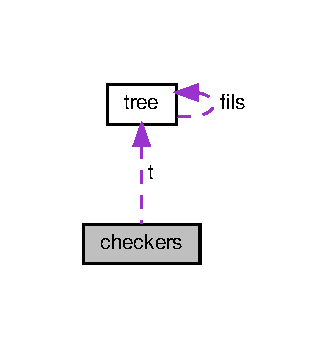
\includegraphics[width=159pt]{structcheckers__coll__graph}
\end{center}
\end{figure}
\subsection*{Public Attributes}
\begin{DoxyCompactItemize}
\item 
\mbox{\Hypertarget{structcheckers_ab10916b6aa2e96e60894cba6e474b808}\label{structcheckers_ab10916b6aa2e96e60894cba6e474b808}} 
int {\bfseries board} \mbox{[}10\mbox{]}\mbox{[}10\mbox{]}
\item 
\mbox{\Hypertarget{structcheckers_a602ad9c7b440f44668c7a98f5a654ece}\label{structcheckers_a602ad9c7b440f44668c7a98f5a654ece}} 
int {\bfseries player}
\item 
\mbox{\Hypertarget{structcheckers_a91ece653d57630f0064c1762177bfa79}\label{structcheckers_a91ece653d57630f0064c1762177bfa79}} 
int {\bfseries end}
\item 
\mbox{\Hypertarget{structcheckers_aeb38744d7954f8e5042700f94104ccac}\label{structcheckers_aeb38744d7954f8e5042700f94104ccac}} 
int {\bfseries stock1}
\item 
\mbox{\Hypertarget{structcheckers_a1fa5cb67c7f1d869fc424a291337c3d8}\label{structcheckers_a1fa5cb67c7f1d869fc424a291337c3d8}} 
int {\bfseries stock2}
\item 
\mbox{\Hypertarget{structcheckers_a439ce9622ed4b69244de32f0f99c1f61}\label{structcheckers_a439ce9622ed4b69244de32f0f99c1f61}} 
int {\bfseries queen1}
\item 
\mbox{\Hypertarget{structcheckers_a6de1957091a2737d691a319f162894dc}\label{structcheckers_a6de1957091a2737d691a319f162894dc}} 
int {\bfseries queen2}
\item 
\mbox{\Hypertarget{structcheckers_a90835a5394c5ada9be5947ee5a0591f9}\label{structcheckers_a90835a5394c5ada9be5947ee5a0591f9}} 
\hyperlink{structtree}{tree} $\ast$ {\bfseries t}
\item 
\mbox{\Hypertarget{structcheckers_a8d727b3458a08691bb33daf8222e2abe}\label{structcheckers_a8d727b3458a08691bb33daf8222e2abe}} 
int {\bfseries score}
\end{DoxyCompactItemize}


The documentation for this struct was generated from the following file\+:\begin{DoxyCompactItemize}
\item 
checkers.\+h\end{DoxyCompactItemize}

\hypertarget{structmove}{}\section{move Struct Reference}
\label{structmove}\index{move@{move}}
\subsection*{Public Attributes}
\begin{DoxyCompactItemize}
\item 
\mbox{\Hypertarget{structmove_a82fd358fe29667cebb87096a754b433a}\label{structmove_a82fd358fe29667cebb87096a754b433a}} 
int {\bfseries x1}
\item 
\mbox{\Hypertarget{structmove_ad8d843eeeadb35673bb508da295433ab}\label{structmove_ad8d843eeeadb35673bb508da295433ab}} 
int {\bfseries y1}
\item 
\mbox{\Hypertarget{structmove_aa9f1f08e972a8bd79a4325dca220127a}\label{structmove_aa9f1f08e972a8bd79a4325dca220127a}} 
int {\bfseries x2}
\item 
\mbox{\Hypertarget{structmove_ac7da4e07393e4438d4dcddb7cd7e3377}\label{structmove_ac7da4e07393e4438d4dcddb7cd7e3377}} 
int {\bfseries y2}
\item 
\mbox{\Hypertarget{structmove_abdb263d0a792f735f3c1c490573a7e4e}\label{structmove_abdb263d0a792f735f3c1c490573a7e4e}} 
int {\bfseries type\+\_\+piece}
\item 
\mbox{\Hypertarget{structmove_a03b45f81cd9e8e87ba9cfe9bafdb4066}\label{structmove_a03b45f81cd9e8e87ba9cfe9bafdb4066}} 
int {\bfseries prise}
\item 
\mbox{\Hypertarget{structmove_a9222355305b5612b700a366d71995f58}\label{structmove_a9222355305b5612b700a366d71995f58}} 
int {\bfseries x3}
\item 
\mbox{\Hypertarget{structmove_a26f2b3d8c49986724741783bfb346582}\label{structmove_a26f2b3d8c49986724741783bfb346582}} 
int {\bfseries y3}
\end{DoxyCompactItemize}


The documentation for this struct was generated from the following file\+:\begin{DoxyCompactItemize}
\item 
checkers.\+h\end{DoxyCompactItemize}

\hypertarget{structtree}{}\section{tree Struct Reference}
\label{structtree}\index{tree@{tree}}


Collaboration diagram for tree\+:\nopagebreak
\begin{figure}[H]
\begin{center}
\leavevmode
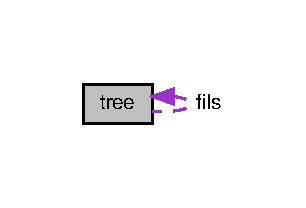
\includegraphics[width=147pt]{structtree__coll__graph}
\end{center}
\end{figure}
\subsection*{Public Attributes}
\begin{DoxyCompactItemize}
\item 
\mbox{\Hypertarget{structtree_adc025a79b084631c7cb73e195fef1b0e}\label{structtree_adc025a79b084631c7cb73e195fef1b0e}} 
int {\bfseries x}
\item 
\mbox{\Hypertarget{structtree_a1703e04257facd6c26ec7a0b2d70e20b}\label{structtree_a1703e04257facd6c26ec7a0b2d70e20b}} 
int {\bfseries y}
\item 
\mbox{\Hypertarget{structtree_acc1638e62e8bb9c8e641625d6cd08a64}\label{structtree_acc1638e62e8bb9c8e641625d6cd08a64}} 
int {\bfseries nbfils}
\item 
\mbox{\Hypertarget{structtree_ac7510e2957091159e3697437d7a7d283}\label{structtree_ac7510e2957091159e3697437d7a7d283}} 
int {\bfseries score}
\item 
\mbox{\Hypertarget{structtree_a74a64c65df6fd5c2df44cf47c83ba6d6}\label{structtree_a74a64c65df6fd5c2df44cf47c83ba6d6}} 
struct \hyperlink{structtree}{tree} $\ast$ {\bfseries fils} \mbox{[}20\mbox{]}
\end{DoxyCompactItemize}


The documentation for this struct was generated from the following file\+:\begin{DoxyCompactItemize}
\item 
checkers.\+h\end{DoxyCompactItemize}

%--- End generated contents ---

% Index
\backmatter
\newpage
\phantomsection
\clearemptydoublepage
\addcontentsline{toc}{chapter}{Index}
\printindex

\end{document}
